\documentclass[fontsize=8pt,paper=a4,paper=landscape,twoside=false,parskip=half,
headings=small,numbers=withenddot,usegeometry=true,english]{scrartcl}

% Packages que conozco
\usepackage[T1]{fontenc} % Necesario para acceder a caracteres especiales
%\usepackage{lmodern} % Fuentes
\usepackage{upgreek} % Caracteres especiales (\uptau, etc.)
%\usepackage[utf8x]{inputenc} % IDEM
\usepackage[english]{babel} % Idioma principal del documento
\usepackage[table,usenames,dvipsnames]{xcolor} % Colores extra para las fuentes
\usepackage{graphicx} % Insertar imágenes
\usepackage{geometry} % Tamaño de Página y Márgenes
\usepackage{enumitem,pifont,textcomp} % Enumerar (letras, números, símbolos, etc.)
\usepackage{multicol} % Texto en columnas
\usepackage{titlesec} % Editar más fácilmente los colores de secciones, subseccinoes, etc.
\usepackage{empheq} % Attractive Boxed Equations
\usepackage[thinc]{esdiff} % Shorthand derivatives
\usepackage{subcaption} % Para poner figuras al lado de las otras
\usepackage{lipsum}

% Configuración de algunos packages que conozco
\geometry{paper=a4paper,landscape, left=6mm,right=6mm, top=6mm,bottom=4mm}

% Otros packages
%\usepackage{cmbright}
\usepackage[scaled=.90]{beramono}
\usepackage{tabulary}
\usepackage{booktabs}
\usepackage{microtype}
\usepackage{pdfpages}
\usepackage[autostyle=true]{csquotes}	
\usepackage{amsmath,amsthm, amssymb,nicefrac}
\usepackage{mathtools} % ???
\usepackage[sticky-per=true,per-mode=fraction]{siunitx}
\usepackage{float}

% Plots & Graphs
\usepackage{pgfplots}
	\usetikzlibrary{
		calc,
		patterns,
		positioning
	}
	\pgfplotsset{
		compat=1.16,
		samples=200,
		clip=false,
		1Quad/.style={
			axis x line=middle,
			axis y line=middle,
			legend pos=outer north east,
			axis line style={->},
			legend style={font=\tiny},
			label style={font=\tiny},
			tick label style={font=\tiny},
			xlabel style={at={(ticklabel* cs:1)},anchor=west,font=\tiny,},
			ylabel style={at={(ticklabel* cs:1)},anchor=west,font=\tiny,},
			%xlabel=$X$,
			%ylabel=$Y$
			},
		4Quad/.style={
			axis x line=middle,
			axis y line=middle,
			legend pos=outer north east,
			axis line style={->},
			legend style={font=\tiny},
			label style={font=\tiny},
			tick label style={font=\tiny},
			xlabel style={at={(ticklabel* cs:1)},anchor=west,font=\tiny,},
			ylabel style={at={(ticklabel* cs:1)},anchor=west,font=\tiny,}
			},
	}
	\tikzset{
		>=stealth
	}
\usetikzlibrary{math, angles, quotes, arrows.meta}

% Configuración que conozco
\setlist{noitemsep,itemindent=0pt,leftmargin=1.6em,nosep}
\setlist[itemize]{label*=\ding{223}}

% Otra Configuración
\arrayrulecolor{gray!60}
\pagestyle{empty}
\abovedisplayskip=1pt\belowdisplayskip=0pt\abovedisplayshortskip=0pt\belowdisplayshortskip=0pt

% Bibliography (here for listings only)
\usepackage[backend=biber,style=verbose]{biblatex}

% Boxes
\providecommand{\titlebox}[1]{
	\fboxsep0.5em\hspace{-2.0\fboxsep}
	\fcolorbox{BrickRed}{BrickRed}{\parbox{\columnwidth}{\raggedright #1}}
}

\providecommand{\sectionbox}[1]{\fboxsep0.5em\hspace*{-1.5\fboxsep}%
 \fcolorbox{gray}{gray!3}{%
 \parbox{\columnwidth}{%
 \raggedright #1}}}
 
\providecommand{\examplebox}[1]{\fboxsep0.5em\hspace*{-1.5\fboxsep}%
 \fcolorbox{gray}{Goldenrod!15!white!}{%
 \parbox{\columnwidth}{%
 \raggedright #1}}}

% Espacio entre párrafos
\setlength{\parskip}{2pt}
\renewcommand{\arraystretch}{2}
\renewcommand{\baselinestretch}{1}

% Configuraciones de tablas
\setlength{\tabcolsep}{3pt}

% Fuente de secciones y subsecciones
%\setkomafont{disposition}{\color{Blue}} % Creo que esto es un comando total, para todo
\setkomafont{section}{\LARGE\bfseries\color{White}}
\setkomafont{subsection}{\large\bfseries\color{BrickRed}}
\setkomafont{subsubsection}{\footnotesize\normalfont\bfseries\color{Mahogany}}

%\renewcommand*{\thesection}{\Alph{section}}
\setcounter{secnumdepth}{0}
\RedeclareSectionCommand[beforeskip=1pt, afterskip=5sp]{section}
\RedeclareSectionCommand[beforeskip=-2pt, afterskip=3sp]{subsection}
\RedeclareSectionCommand[beforeskip=-2pt, afterskip=3sp]{subsubsection}


% Path para las imágenes
\graphicspath{{img/}}

% Cprotect =====================================================================================
\usepackage{cprotect}
\def\AAAfoldernamecprotect{cpt_files} % Name of the folder in which .cpt files are stored

\makeatletter % This block is necessary implements the new destination of .cpt files
  \def\CPT@read@mbeg{%
  \stepcounter{CPT@WriteCount}%
  \edef\CPT@filename{./\AAAfoldernamecprotect/\jobname-\arabic{CPT@WriteCount}.cpt}%
  \expandafter\expandafter\expandafter\CPT@commandatend@toks
  \expandafter\expandafter\expandafter{%
    \expandafter\the
    \expandafter\CPT@commandatend@toks
    % Input a file:
    \expandafter{%
      \expandafter\protect
      \expandafter\input
      \CPT@filename
      \relax
    }%
  }%
  %\showthe\CPT@commandatend@toks%
  \begingroup%
  \makeallother%
  \def\CPT@preText{}%
  \let\CPT@postText\CPT@hat@hat@E@hat@hat@L%
  \let\CPT@begin\CPT@other@bgroup%
  \let\CPT@end\CPT@other@egroup%
  \CPT@readContent%
}%
\makeatother

% make boxes robust for verbatim
\let\oldsectionbox\sectionbox
\outer\def\sectionbox{\icprotect\oldsectionbox}

% Hyperref =====================================================================================
\usepackage{hyperref}
\renewcommand{\subsectionautorefname}{section}

\definecolor{darkblue}{RGB}{0, 82, 147}		
\hypersetup{
	pdfcreator={LaTeX2e},
	pdfborder=0 0 0,
	breaklinks=true,
	bookmarksopen=true,
	bookmarksnumbered=true,
	linkcolor=darkblue,
	urlcolor=darkblue,
	citecolor=darkblue,
	colorlinks=true,
	pdfauthor=Marion Lammarsch, 
	pdftitle=LaTeX Cheat Sheet,
	pdfcreator=LaTeX2e 
}
\urlstyle{sf}

% Source Code Listings ============
\usepackage{listings}
\lstset{
	backgroundcolor=\color{listinggray},
	basicstyle=\ttfamily\small,
	aboveskip={0.4\baselineskip},
	belowskip={0.4\baselineskip},
	literate={ä}{{\"a}}1 {ö}{{\"o}}1 {ü}{{\"u}}1 {Ä}{{\"A}}1 {Ö}{{\"O}}1 {Ü}{{\"u}}1 {ß}{{\ss}}1 {ô}{{\^o}}1	
}

\lstnewenvironment{mylatex} 
{\lstset{%
	backgroundcolor=\color{listinggray},
	%basicstyle=\ttfamily\small,
	tabsize=2,
	language={[LaTeX]TeX},
	%upquote=true,
	aboveskip={0.4\baselineskip},
	belowskip={0.4\baselineskip},
	abovecaptionskip={\baselineskip},
	belowcaptionskip={0\baselineskip},
	columns=fixed,
	showstringspaces=false,
	extendedchars=true,
	linewidth=.96\linewidth,
	xleftmargin=.04\linewidth,
	frameround=fttt,
	framexleftmargin={2pt},
	framexrightmargin={2pt},
	prebreak = \raisebox{0ex}[0ex][0ex]{\ensuremath{\hookleftarrow}},
	frame=single,
	showtabs=false,
	showspaces=false,
	showstringspaces=false,
	identifierstyle=\ttfamily,
	keywordstyle=\color{darkblue},
	commentstyle=\color[rgb]{0.133,0.545,0.133},
	stringstyle=\color[rgb]{0.8,  0.1,  0.1},
	morekeywords={part,chapter,subsection,subsubsection,paragraph,subparagraph,tableofcontents,%
		listoffigures,listoftables,printacronyms,ihead,ohead,clearscrheadings,clearmainofpairofpagestyles,%
		headmark,pagemark,maketitel,tr,varnothing,renewcommand,usepackage,includegraphics,graphicspath,%
		acsetup,DeclareAcroListStyle,DeclareAcronym,ac,Ac,definecolor,colorlet,textcolor,colorbox,%
		rowcolor,addbibresource,autocite,printbibliography,%	
		nexists,KOMAoptions,PassOptionsToPackage,thesection,thefigure,color,foreignlanguage},
	literate={ä}{{\"a}}1 {ö}{{\"o}}1 {ü}{{\"u}}1 {Ä}{{\"A}}1 {Ö}{{\"O}}1 {Ü}{{\"u}}1 {ß}{{\ss}}1 {ô}{{\^o}}1	
}}{}

\sloppy

% Macros y Nuevos comandos
\newcommand{\topline}{\vspace{2pt}{\color{Gray!80}\hrule}\vspace{3pt}}
\renewcommand{\qedsymbol}{$\blacksquare$}


% Distancia antes y después de cada {figure}
\setlength{\intextsep}{5pt plus 2pt minus 2pt}

\usepackage{fontspec}
\setmainfont{Revx Neue Demo}

% DOCUMENT_BEGINS ====================================================================================
\begin{document}

% FIRST 4 COLS
\begin{multicols*}{4}

\parbox{\columnwidth}{\centering\Huge\color{Black}\textbf{SCMx1 \strut}}\scriptsize

\titlebox{\section{TITLE 1}}

\subsection{What is a Supply Chain?}

\sectionbox{
Suppliers, Producers, Customers. TEST}

\sectionbox{
In a manufacturing context, a supply chain can be seen as a network of suppliers, manufacturers, distributors, and retailers
}

\sectionbox{\subsubsection{Network Model}\topline
EOQ formula:

\[ Q^* = \sqrt{\frac{ABC}{D}} \]

}

\sectionbox{\subsubsection{Flows}\topline
\begin{figure}[H]
	\centering
	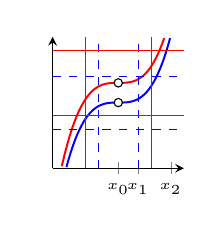
\begin{tikzpicture}
	\begin{axis}[1Quad,width=3.25cm,height=3.25cm,ymin=0,ymax=2,xmin=0,xmax=2, 
				ytick style={draw=none},
				xtick={1,1.3,1.8}, xticklabels={$x_{0}$, $x_{1}$, $x_{2}$}, yticklabels={,,},
				restrict y to domain = 0:2]
		% Function and e-d limits
		\addplot[blue, line width=0.25mm, domain=0:2]{2*(x-1)^3+1};
		\addplot[red, line width=0.25mm, domain=0:2]{2*(x-1)^3+1.3};
		\draw (0.7,0)node[]{}--(0.7,2)node[]{}[blue, dashed, line width=0.05mm];
		\draw (1.3,0)node[]{}--(1.3,2)node[]{}[blue, dashed, line width=0.05mm];
		\draw (0,0.6)node[]{}--(2,0.6)node[]{}[blue, dashed, line width=0.05mm];
		\draw (0,1.4)node[]{}--(2,1.4)node[]{}[blue, dashed, line width=0.05mm];
		\draw (0.5,0)node[]{}--(0.5,2)node[]{}[red, line width=0.10mm];
		\draw (1.5,0)node[]{}--(1.5,2)node[]{}[red, line width=0.10mm];
		\draw (0,0.8)node[]{}--(2,0.8)node[]{}[red, line width=0.10mm];
		\draw (0,1.8)node[]{}--(2,1.8)node[]{}[red, line width=0.10mm];
		% White dot
		\node[circle,draw=black,fill=white,inner sep=0pt,minimum size=3pt] at (1,1) {};
		\node[circle,draw=black,fill=white,inner sep=0pt,minimum size=3pt] at (1,1.3) {};
	\end{axis}
	\end{tikzpicture}
	\hspace{0.25cm}
	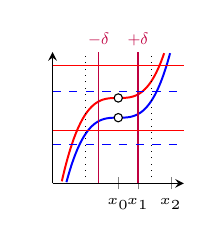
\begin{tikzpicture}
	\begin{axis}[1Quad,width=3.25cm,height=3.25cm,ymin=0,ymax=2,xmin=0,xmax=2, 
				ytick style={draw=none},
				xtick={1,1.3,1.8}, xticklabels={$x_{0}$, $x_{1}$, $x_{2}$}, yticklabels={,,},
				restrict y to domain = 0:2]
		% Function and e-d limits
		\addplot[blue, line width=0.25mm, domain=0:2]{2*(x-1)^3+1};
		\addplot[red, line width=0.25mm, domain=0:2]{2*(x-1)^3+1.3};
		\draw (0.7,0)node[]{}--(0.7,2)node[purple,above,scale=0.6]{$-\delta$}[purple,line width=0.15mm];
		\draw (1.3,0)node[]{}--(1.3,2)node[purple,above,scale=0.6]{$+\delta$}[purple,line width=0.15mm];
		\draw (0,0.6)node[]{}--(2,0.6)node[]{}[blue, dashed, line width=0.05mm];
		\draw (0,1.4)node[]{}--(2,1.4)node[]{}[blue, dashed, line width=0.05mm];
		\draw (0.5,0)node[]{}--(0.5,2)node[]{}[black, dotted, line width=0.10mm];
		\draw (1.5,0)node[]{}--(1.5,2)node[]{}[black, dotted, line width=0.10mm];
		\draw (0,0.8)node[]{}--(2,0.8)node[]{}[red, line width=0.10mm];
		\draw (0,1.8)node[]{}--(2,1.8)node[]{}[red, line width=0.10mm];
		% White dot
		\node[circle,draw=black,fill=white,inner sep=0pt,minimum size=3pt] at (1,1) {};
		\node[circle,draw=black,fill=white,inner sep=0pt,minimum size=3pt] at (1,1.3) {};
	\end{axis}
	\end{tikzpicture}
\end{figure}
}

\subsection{What is Supply Chain Management?}

\sectionbox{\subsubsection{SCM Activities}\topline

}

\titlebox{\section{TITLE 2}}

\subsection{Subtitle 2}

\sectionbox{\subsubsection{Subsubtitle 2}\topline

}

\end{multicols*}

\newpage

Holass

\end{document}